\chapter{Methodology}
\section{Software Development Approach}
 is an iterative process-based approach to software development. In the Agile process model, work is broken down into more manageable, smaller iterations without requiring a lot of long-term planning. The requirements and scope of the project are determined early on, and the number, length, and scope of each iteration are preplanned. Each iteration is considered as a short time "frame" in the Agile process model, which lasts for a few weeks. In each iteration, teams move through the phases of the software development life cycle, which include planning, requirements analysis, design, coding, testing, and demonstration of a working product for client review. Agile places a significant value on flexibility, teamwork, and regular client feedback.\\
\begin{figure}[H]
    \centering
    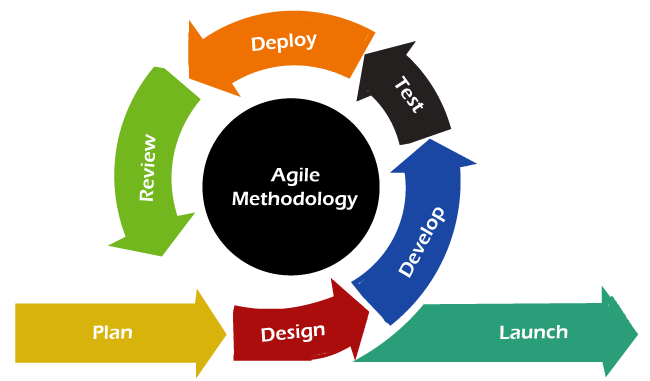
\includegraphics[width=80mm]{./img/agile.png}
    \caption{Agile Model}
\end{figure}
The main reason for which  we choose this development process:
\begin{enumerate}[noitemsep] %label=\Roman*.]
\item Very quick,flexible and efficient.
\item Risk minimization.
\item Projects are split into sprints for better management and productivity.
\item Through iterative testing and sprints, the final product contains less bugs. 
\item Development period for application is reduced.
\end{enumerate}
\begin{figure}[H]
\section {Block diagram of proposed system}
% \centering
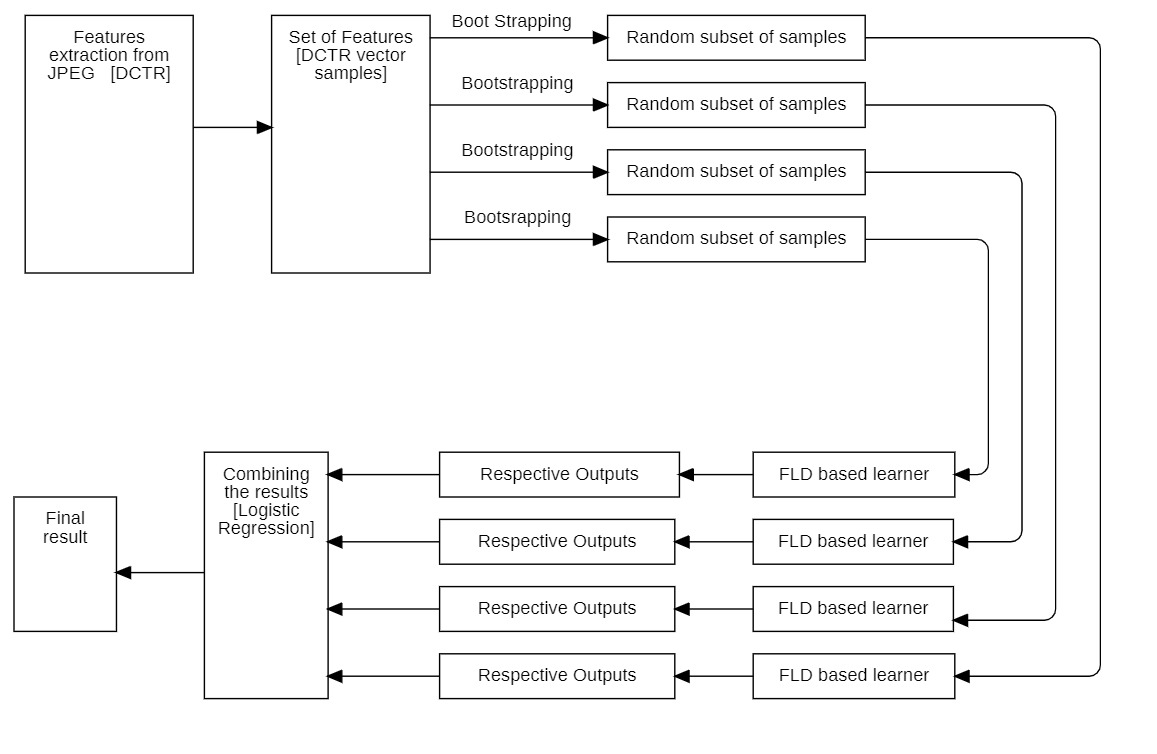
\includegraphics[width=1.1\textwidth]{./img/block_d.jpg}\\
\caption{ Block diagram of proposed system}
\end{figure}
\clearpage

\begin{flushleft}
    \Large{\textbf{Model Training Approach}}\\
\end{flushleft}
\textbf{Feature Extraction:}\\
Initial extraction of DCTR (Discrete Cosine Transform Ratio) feature vector from images or.jpeg files is to be done. The selection of DCTR is based on its detection efficiency in comparison to other parameters such as PHARM and GFR.\vspace{0.25cm}\\
\textbf{Ensemble Classifier Selection:}\\
The decision to choose ensemble classifiers over deep learning techniques was made due to their superior steganalysis detection efficiency and their need for lesser computational power.\vspace{0.25cm}\\
\textbf{Bootstrapping:}\\
Bootstrapping is the process of splitting a large dataset into its smaller subsets. The gathered DCTR feature vectors are to be split  into more manageable subsets. Utilizing these subsets, individual base models are to be trained independently.\vspace{0.25cm}\\
\textbf{Base Learner Training:}\\
Based on the extracted features, each base learner independently processes its subset of feature vectors and finalizes a decision.\vspace{0.25cm}\\
\textbf{Aggregation:}\\
To create an ensemble decision, the choices made by each individual base learner are aggregated and the final decision is to be made by using a voting system which finalizes the result by figuring out the most popular output.\vspace{0.25cm}\\
\textbf{Efficiency Considerations:}\\
The proposed system prioritizes efficiency by leveraging shallow machine learning techniques, particularly ensemble classifiers instead of deep learning. The choice of DCT as a feature is intentional to increase efficiency and detection capability of the system.\\
\clearpage 

\section{System Architecture}
\begin{figure}[H]
    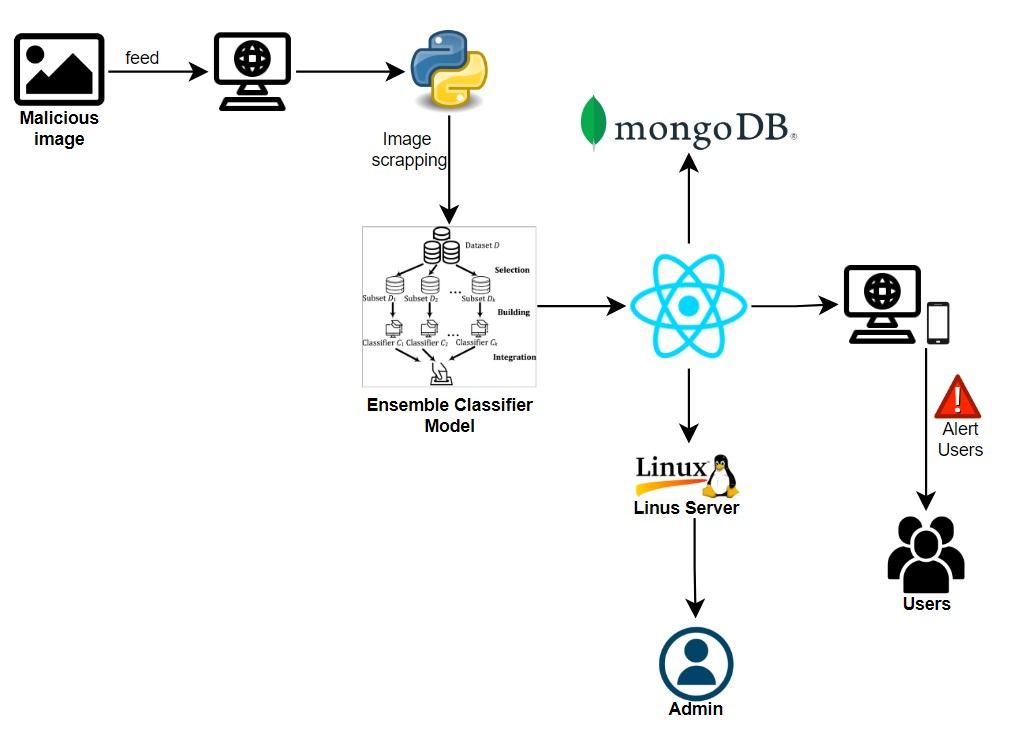
\includegraphics[width=180mm]{./img/System architecture.jpg}
    \caption{System Architecture}
\end{figure}
\clearpage 
